\chapter{Random Variables}


We model stock returns as \textit{random variables}.
A random variable can take one of many values, with an 
associated probability. For example, the gross return on 
a stock can be one of four values as shown in Table \ref{tab:randomvariable}.

\begin{table}[!htbp]
    \centering
    \begin{tabular}{c c}
        % \hline
        $R$ & $P(R)$ \\
        % \hline
        1.1 & 0.6 \\
        1.2 & 0.1 \\
        0.7 & 0.25 \\
        0.0 & 0.05 \\
    \end{tabular}
    \caption{Example of a gross return distribution.}
    \label{tab:randomvariable}
\end{table}

Each value is a possible \textit{realization}
of the random variable. You can experiment with this in Python
using the following code:

\begin{python}
import numpy as np

# Define the possible returns and their probabilities
returns = np.array([1.1, 1.2, 0.7, 0.0])
probabilities = np.array([0.6, 0.1, 0.25, 0.05])

# Generate a random return
print(np.random.choice(returns, size=1, p=probabilities))

\end{python}

Of course, stock returns can take on many more values 
than just four, but this is a simple example.

The \textit{distribution} of the random variable is 
a listing of the values it can take, along with their
associated probabilities. For example, the distribution
of the random variable in Table \ref{tab:randomvariable}
is:

\begin{figure}[!htbp]
    \centering
    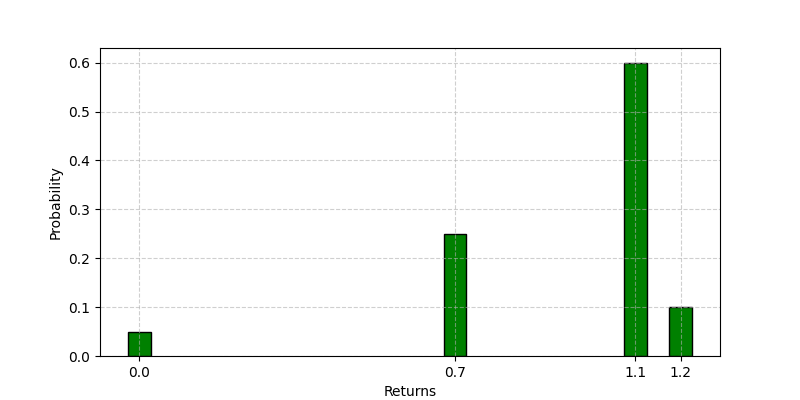
\includegraphics[width=0.8\textwidth]{randomvariables/fig1.png}
    \caption{Example of a random variable distribution.}
    \label{fig:randomvariable}
\end{figure}

Another way to think of a random variable is as a
\textit{function} that maps "states of the world" to
real numbers. For example, the random variable in 
Table \ref{tab:randomvariable} could be:

\begin{table}[!htbp]
    \centering
    \begin{tabular}{c c c}
        % \hline
        $R$ & States of the world & $P(R)$ \\
        % \hline
        1.1 & New product works, competitor burns down & 0.6 \\
        1.2 & New product works, competitor ok. & 0.1 \\
        0.7 & Only old products work & 0.25 \\
        0.0 & Factory burns down, no insurance. & 0.05 \\
    \end{tabular}
    \caption{Random variable as a function mapping states of the world to real numbers.}
    \label{tab:statesoftheworld}
\end{table}

The probability really describes the external events 
that define the states of the world. Usually, we 
can't name those events, so we just use the probabilities
that the stock return takes on various values.